%\documentclass[10pt,notes]{beamer}       % print frame + notes
%\documentclass[10pt, notes=only]{beamer}   % only notes
\documentclass[11pt]{beamer}              % only frames

%%%%%% IF YOU WOULD LIKE TO CREATE LECTURE NOTES COMMENT OUT THE FOlLOWING TWO LINES
%\usepackage{pgfpages}
%\setbeameroption{show notes on second screen=bottom} % Both

\usepackage{graphicx}
\DeclareGraphicsExtensions{.pdf,.png,.jpg}
\usepackage{color}
\usetheme{winslab}
\usepackage[utf8]{inputenc}
\usepackage[english]{babel}
\usepackage{amsmath}
\usepackage{amsfonts}
\usepackage{amssymb}




\usepackage{algorithm2e,algorithmicx,algpseudocode}
\algnewcommand\Input{\item[\textbf{Input:}]}%
\algnewcommand\Output{\item[\textbf{Output:}]}%
\newcommand\tab[1][1cm]{\hspace*{#1}}

\algnewcommand{\Implement}[2]{\item[\textbf{Implements:}] #1 \textbf{Instance}: #2}%
\algnewcommand{\Use}[2]{\item[\textbf{Uses:}] #1 \textbf{Instance}: #2}%
\algnewcommand{\Trigger}[1]{\Statex{\textbf{Trigger:} (#1)}}%
\algnewcommand{\Events}[1]{\item[\textbf{Events:}] #1}%
\algnewcommand{\Need}[1]{\item[\textbf{Needs:}] #1}%
\algnewcommand{\Event}[2]{\Statex \item[\textbf{On#1:}](#2) \textbf{do}}%
\algnewcommand{\Trig}[3]{\State \textbf{Trigger}  #1.#2 (#3) }%
\def\true{\textbf{T}}
\def\false{\textbf{F}}


\author[Ahmet Kürşad Şaşmaz]{Ahmet Kürşad Şaşmaz\\\href{mailto:kursad.sasmaz@metu.edu.tr}{kursad.sasmaz@metu.edu.tr}}
%\author[J.\,Doe \& J.\,Doe]
%{%
%  \texorpdfstring{
%    \begin{columns}%[onlytextwidth]
%      \column{.45\linewidth}
%      \centering
%      John Doe\\
%      \href{mailto:john@example.com}{john@example.com}
%      \column{.45\linewidth}
%      \centering
%      Jane Doe\\
%      \href{mailto:jane.doe@example.com}{jane.doe@example.com}
%    \end{columns}
%  }
%  {John Doe \& Jane Doe}
%}

\title[Ricart-Argawala Algorithm]{Ricart-Argawala Algorithm}
\subtitle[Mutual Exclusion in Distributed Systems]{Mutual Exclusion in Distributed Systems}
%\date{} 

\begin{document}

\begin{frame}[plain]
\titlepage
\note{In this talk, I will present .... Please answer the following questions:
\begin{enumerate}
\item Why are you giving presentation?
\item What is your desired outcome?
\item What does the audience already know  about your topic?
\item What are their interests?
\item What are key points?
\end{enumerate}
}
\end{frame}

\begin{frame}[label=toc]
    \frametitle{Outline of the Presentation}
    \tableofcontents[subsubsectionstyle=hide]
\note{ The possible outline of a talk can be as follows.
\begin{enumerate}
\item Outline 
\item Problem and background
\item Design and methods
\item Major findings
\item Conclusion and recommendations 
\end{enumerate} Please select meaningful section headings that represent the content rather than generic terms such as ``the problem''. Employ top-down structure: from general to more specific.
}
\end{frame}
%
%\part{This the First Part of the Presentation}
%\begin{frame}
%        \partpage
%\end{frame}
%
\section{The Problem}
%\begin{frame}
%        \sectionpage
%\end{frame}

\begin{frame}{The Problem}
\framesubtitle{Selecting owner of a resource without any conflict}
\begin{block}{Mutual Exclusion in Distributed Systems} 
Mutual exclusion in distributed systems refers to the challenge of properly accessing a shared resource at any given time by different concurrent processes on different machines. The motivation is ensuring that only one process holds the resource and this resource is orderly accessed for all participants in the system by using coordination and synchronization systems.
\end{block}
\note{}
\end{frame}

\section{Our Motivation}
\begin{frame}
\frametitle{Our Motivation}
\framesubtitle{It is better to declare everyone that you wanted first.}
Imagine a server with limited CPUs. And as having a bad CEO, the only communication channel for prioritizing users is a chat application. You and your co-workers are agreed on some rules:
\begin{itemize}
    \item If someone requests the resource, the ones are not using and the ones are not currently interested in using will reply "OK!" immediately.
    \item If someone has things to do with the resource but not wanted first is also reply as "OK!"
    \item No one can use the resource without ensuring that no one is currently interested or using.
    \item Anyone has to inform the concerned ones in the time of using the resource after releasing it
\end{itemize}
\end{frame}
\note{}

\section{The Proposed Solution}
\begin{frame}
\frametitle{The Proposed Solution}
\framesubtitle{}

This innovative approach tackles the complexities of coordinating critical section access across multiple nodes, overcoming hurdles like network communication and synchronization. Using timestamps to guide communication, this algorithm elegantly orchestrates interactions between nodes, guaranteeing smooth and fair resource sharing.

That has advantages in terms of:

\begin{itemize}
\item Communication efficiency
\item Message complexity
\item Timestamp prioritization
\end{itemize}

\end{frame}


\section{Background Information and Previous Works}


\subsection{Background Information}

\frame{
\frametitle{Background Information}
In distributed systems, mutual exclusion is crucial for preventing race conditions, ensuring that only one process can
access a critical section at any given time.

Requirements for a mutual exclusion algorithm in distributed systems are:
\begin{itemize}
    \item \textbf{No Deadlock:} Ensure processes don’t indefinitely wait for messages.
    \item \textbf{No Starvation:} Every process should have a chance to execute its critical section in finite time.
    \item \textbf{Fairness:} Requests to execute critical sections should be executed in the order they arrive.
    \item \textbf{Fault Tolerance:} The system should recognize failures and continue functioning without disruption.
\end{itemize}
}

\subsection{Previous Works}
\begin{frame}{Previous Works}

Previous works are based on different methods.

\begin{itemize}
    \item \textbf{Token Based Algorithm:} Uses a unique token shared among sites, allowing possession of the token to enter the critical section. Examples include the Suzuki-Kasami Algorithm and Raymond’s Algorithm.
    \item \textbf{Non-token based approach:} Sites communicate to determine which should execute the critical section next, using timestamps to order requests. Examples include the Ricart-Agrawala Algorithm explained in this presentation.
    \item \textbf{Quorum based approach:} Sites request permission from a subset called a quorum, ensuring mutual exclusion through common subsets. Examples include Maekawa’s Algorithm.
\end{itemize}

\end{frame}




\section{The Algorithm}
\subsection{Algorithm Description}
\begin{frame}{Algorithm Description}
Ricart-Argawala Algorithm is based on fully connected topology. Every node has these features:

\begin{itemize}
    \item Connection to every other nodes
    \item Timestamp prioritization
\end{itemize}

\end{frame}


\subsection{Pseudocode}

\begin{frame}
\frametitle{Algorithm Pseudocode Part 1}

\begin{center}
\begin{algorithm}[H]
	\scriptsize
	\def\algorithmlabel{Ricart-Agrawala}
    \caption{\algorithmlabel\ algorithm}
    \label{alg:ricart_agrawala}
    \begin{algorithmic}[1]
    	\Implement {\algorithmlabel}{cf} 
        \Use {Integer} {self\_id}
    	\Use {List of Requests} {deferred\_requests} 
    	\Use {Set of Nodes} {other\_nodes} 
    	\Use {Set of Nodes} {nodes\_replied} 
    	\Use {Logical Clock} {request\_clock}
    	\Use {Logical Clock} {clock}
    	\Use {Boolean} {using\_critical\_section}
        \Use {Boolean} {has\_privilege}
        \Use {Boolean} {want\_privilege}
    	\Events{Init, WantUsingCriticalSection, EndUsingCriticalSection, ReceiveRequestMessage, ReceiveReplyMessage}
	   \Need {}
    \end{algorithmic}
\end{algorithm}
\end{center}

\end{frame}

\begin{frame}
\frametitle{Algorithm Pseudocode Part 2}

\begin{center}
\begin{algorithm}[H]
	\scriptsize
	\def\algorithmlabel{Ricart-Agrawala}
    \caption{\algorithmlabel\ algorithm}
    \label{alg:ricart_agrawala}
    \begin{algorithmic}[1]
        \Event {Init}{ }
            \begin{enumerate}
                \item other\_nodes ← topology\_nodes / self\_id
            \end{enumerate}
    \end{algorithmic}
\end{algorithm}
\end{center}
\end{frame}

\begin{frame}
\frametitle{Algorithm Pseudocode Part 3}

\begin{center}
\begin{algorithm}[H]
	\scriptsize
	\def\algorithmlabel{Ricart-Agrawala}
    \caption{\algorithmlabel\ algorithm}
    \label{alg:ricart_agrawala}
    \begin{algorithmic}[1]
        \Event {WantUsingCriticalSection}{ }
            \begin{enumerate}
                \item if want\_privilege = false then
                \item \quad if using\_critical\_section = false then
                \item \quad \quad if has\_privilege = true then
                \item \quad \quad \quad using\_critical\_section ← true;
                \item \quad \quad else then
                \item \quad \quad \quad want\_privilege ← true;
                \item \quad \quad \quad request\_clock ← clock;
                \item \quad \quad \quad clock ← clock + 1;
                \item \quad \quad \quad for node\_id in other\_nodes
                \item \quad \quad \quad send request message including request\_clock to node with node\_id
                \item \quad \quad end for
                \item \quad end if
            \end{enumerate}
    \end{algorithmic}
\end{algorithm}
\end{center}
\end{frame}

\begin{frame}
\frametitle{Algorithm Pseudocode Part 4}

\begin{center}
\begin{algorithm}[H]
	\scriptsize
	\def\algorithmlabel{Ricart-Agrawala}
    \caption{\algorithmlabel\ algorithm}
    \label{alg:ricart_agrawala}
    \begin{algorithmic}[1]
        \Event {EndUsingCriticalSection}{ }
            \begin{enumerate}
                \item using\_critical\_section ← false;
                \item want\_privilege ← false;
                \item clear nodes\_replied
                \item if deferred\_requests is not empty then
                \item \quad has\_privilege ← false;
                \item \quad while deferred\_requests is not empty
                \item \quad \quad pop from deferred\_requests into deferred\_request;
                \item \quad \quad if clock <= deferred\_request.clock then
                \item \quad \quad \quad clock ← deferred\_request.clock + 1
                \item \quad \quad end if
                \item \quad \quad send reply message to node with deferred\_request.node\_id;
                \item \quad end while
                \item end if
            \end{enumerate}
    \end{algorithmic}
\end{algorithm}
\end{center}
\end{frame}

\begin{frame}
\frametitle{Algorithm Pseudocode Part 5}

\begin{center}
\begin{algorithm}[H]
	\scriptsize
	\def\algorithmlabel{Ricart-Agrawala}
    \caption{\algorithmlabel\ algorithm}
    \label{alg:ricart_agrawala}
    \begin{algorithmic}[1]
        \Event {ReceiveRequestMessage}{ }
            \begin{enumerate}
                \item if using\_critical\_section = false then
                \item \quad if has\_privilege = true then
                \item \quad \quad has\_privilege ← false;
                \item \quad \quad if clock <= message.clock then
                \item \quad \quad \quad clock ← message.clock + 1;
                \item \quad \quad end if
                \item \quad \quad send reply message to node with message.node\_id;
                \item \quad else then
                \item \quad \quad if want\_privilege = true then
                \item \quad \quad \quad if request\_clock > message.clock then
                \item \quad \quad \quad \quad if clock <= request\_clock then
                \item \quad \quad \quad \quad \quad clock ← request\_clock + 1;
                \item \quad \quad \quad \quad end if
                \item \quad \quad \quad send reply message to node with message.node\_id;
                \item \quad \quad \quad else then
                \item \quad \quad \quad \quad push $<$message$>$ into deferred\_requests;
                \item \quad \quad \quad end if
                \item \quad \quad else then
                \item \quad \quad \quad if clock <= message.clock then
                \item \quad \quad \quad \quad clock ← message.clock + 1;
                \item \quad \quad \quad end if
                \item \quad \quad \quad send reply message to node with message.node\_id;
                \item \quad \quad end if
                \item \quad endif
                \item else then
                \item \quad push $<$message$>$ into deferred\_requests;
                \item end if
            \end{enumerate}
    \end{algorithmic}
\end{algorithm}
\end{center}
\end{frame}

\begin{frame}
\frametitle{Algorithm Pseudocode Part 6}

\begin{center}
\begin{algorithm}[H]
	\scriptsize
	\def\algorithmlabel{Ricart-Agrawala}
    \caption{\algorithmlabel\ algorithm}
    \label{alg:ricart_agrawala}
    \begin{algorithmic}[1]
        \Event {ReceiveReplyMessage}{ }
            \begin{enumerate}
                \item push $<$i$>$ into nodes\_replied
                \item if nodes\_replied = other\_nodes then
                \item \quad has\_privilege ← true;
                \item \quad using\_critical\_section ← true;
                \item end if
            \end{enumerate}

    \end{algorithmic}
\end{algorithm}
\end{center}
\end{frame}

\begin{frame}
\frametitle{Strength of The Algorithm}
\framesubtitle{Correctness}
\begin{itemize}
    \item \textbf{Mutual Exclusion}
\end{itemize}
\end{frame}

\begin{frame}
\frametitle{Strength of The Algorithm}
\framesubtitle{Complexity}
\begin{itemize}
    \item \textbf{Message Complexity:} $2(N-1)$
    \item \textbf{Memory Complexity:} $N-1$
\end{itemize}
\end{frame}

\section{Experimental results/Proofs}

\subsection{Message Complexity - Node Count \& Edge Probability}
\begin{frame}
\frametitle{Message Complexity - Node Count \& Edge Probability}
\framesubtitle{}
\begin{figure}
    \centering
    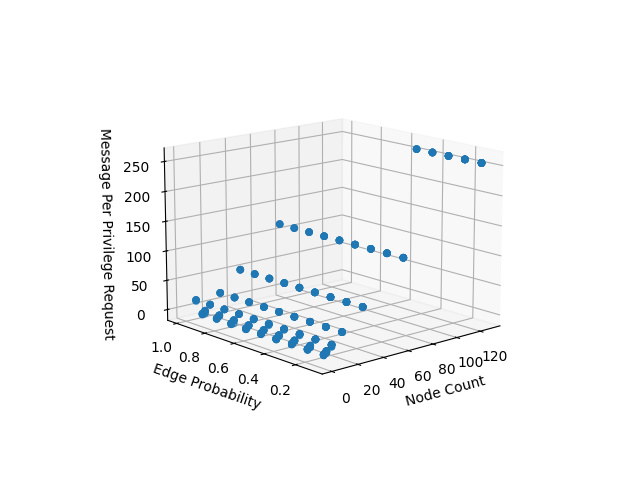
\includegraphics[scale=0.5]{figures/RicartAgrawalaAlgorithmMessageComplexity.png}
    \caption{Ricart Agrawala Algorithm Message Complexity}
    \label{fig:ricart_agrawala_algoritm_message_complexity}
\end{figure}
\end{frame}

\subsection{Forwarded Message Complexity - Node Count \& Edge Probability}
\begin{frame}
\frametitle{Forwarded Message Complexity - Node Count \& Edge Probability}
\framesubtitle{}
\begin{figure}
    \centering
    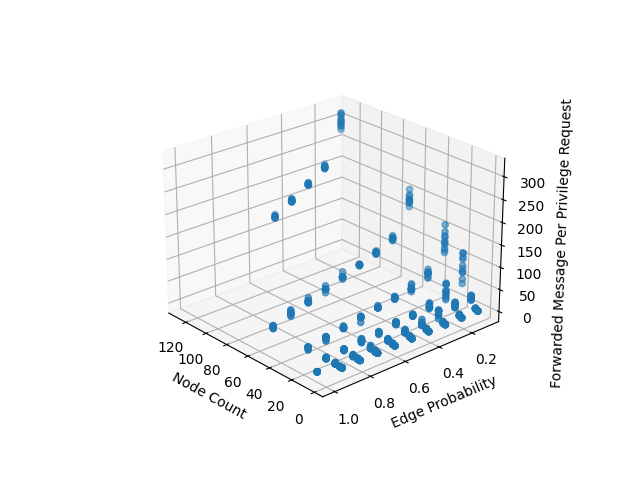
\includegraphics[scale=0.5]{figures/RicartAgrawalaAlgorithmForwardedMessageComplexity.png}
    \caption{Ricart Agrawala Algorithm Forwarded Message Complexity}
    \label{fig:ricart_agrawala_algoritm_forwarded_message_complexity}
\end{figure}
\end{frame}

\section{Conclusions}
\begin{frame}
\frametitle{Conclusions}
\framesubtitle{}
\begin{itemize}
    \item Message Complexity
    \item Memory Complexity
    \item Node Failure
\end{itemize}

\end{frame}

\thankslide

\end{document}